\documentclass{article}

% if you need to pass options to natbib, use, e.g.:
%     \PassOptionsToPackage{numbers, compress}{natbib}
% before loading neurips_2024


% ready for submission
\usepackage{neurips_2024}


% to compile a preprint version, e.g., for submission to arXiv, add add the
% [preprint] option:
%     \usepackage[preprint]{neurips_2024}


% to compile a camera-ready version, add the [final] option, e.g.:
%     \usepackage[final]{neurips_2024}


% to avoid loading the natbib package, add option nonatbib:
%    \usepackage[nonatbib]{neurips_2024}


\usepackage[utf8]{inputenc} % allow utf-8 input
\usepackage[T1]{fontenc}   % use 8-bit T1 fonts
\usepackage{hyperref}       % hyperlinks
\usepackage{url}            % simple URL typesetting
\usepackage{booktabs}       % professional-quality tables
\usepackage{amsfonts}       % blackboard math symbols
\usepackage{nicefrac}       % compact symbols for 1/2, etc.
\usepackage{microtype}      % microtypography
\usepackage{xcolor}   
\usepackage{graphicx}% colors


\title{Bayesian Inference for Gaussian Graphical Models}


% The \author macro works with any number of authors. There are two commands
% used to separate the names and addresses of multiple authors: \And and \AND.
%
% Using \And between authors leaves it to LaTeX to determine where to break the
% lines. Using \AND forces a line break at that point. So, if LaTeX puts 3 of 4
% authors names on the first line, and the last on the second line, try using
% \AND instead of \And before the third author name.


\author{
  David S.~Hippocampus\thanks{Use footnote for providing further information
    about author (webpage, alternative address)---\emph{not} for acknowledging
    funding agencies.} \\
  Department of Computer Science\\
  Cranberry-Lemon University\\
  Pittsburgh, PA 15213 \\
  \texttt{hippo@cs.cranberry-lemon.edu} \\
  % examples of more authors
  % \And
  % Coauthor \\
  % Affiliation \\
  % Address \\
  % \texttt{email} \\
  % \AND
  % Coauthor \\
  % Affiliation \\
  % Address \\
  % \texttt{email} \\
  % \And
  % Coauthor \\
  % Affiliation \\
  % Address \\
  % \texttt{email} \\
  % \And
  % Coauthor \\
  % Affiliation \\
  % Address \\
  % \texttt{email} \\
}


\begin{document}


\maketitle


\begin{abstract}
  The project aims to apply techniques of Gaussian Graphical Models, a powerful probabilistic tool for modeling and representing conditional dependencies among variables in Multivariate Gaussian Distributions. The current project also aims to introduce a Bayesian Inference perspective via estimation of the Precision matrix via a Gibbs sampling algorithm. The project aims to use these techniques with a protein dataset, in an attempt to model relationships among proteins for patients diagnosed with AML. Our implementation of the Gibbs algorithm found a highly interconnected protein network in the data set, and a viable estimate of the Multivariate Gaussian precision matrix. 
\end{abstract}


\section{Introduction}

\subsection{Literature Review}

Gaussian Graphical Models are used in a variety of contexts to gain a deeper understanding of features and random variables, in this case variables following a Multivariate Gaussian Distribution. This technique's ability to model conditional dependence among many variables in a high-dimensional modeling scenario. 

In particular with proteins and AML, literature suggests a relationship between protein profiling and AML outcomes, particularly response and survival. Given the high-dimensional nature of the data, directly sampling and deriving inference from the posterior distribution will prove difficult. To that end, we utilize a Gibbs sampling algorithm, a special case of the Markov Chain Monte Carlo class of algorithms for posterior distribution estimation via simulation. 

Recent literature suggests a viable method for estimating the precision matrix involves Regression, specifically the Pseudo-Likelihood and Joint regression methods. As is the case with regressions involving high-dimensional data, multicollinearity, variance inflation, and overfitting are consistent problems. 

A way around this in the Bayesian framework involves the Bayesian lasso as well as various prior choices to control parameter magnitude, similar to how shrinkage occurs in Lasso or Ridge regression. 


\subsection{Project Guideline}

The current project aims to integrate these high-dimensional probabilistic techniques and apply them to the AML data set to gain a more intensive understanding of the relationship between proteins for these patients. 

The project will begin with deriving the full conditional distributions to implement the Gibbs sampling algorithm as a way of estimating the precision matrix. The algorithm will be implemented in the usual way, with a burn-in period and specified number of iterations as hyperparameters. 

The estimated Precision matrix will then be used to build the undirected graph from an adjacency matrix, with a 1 or 0 depending on if any two variables (proteins) are conditionally independent or not. 

The resulting undirected graph will serve as a way of modeling the interactions between proteins for these AML patients. That is, any proteins that are connected on the graph can be thought of as conditionally dependent, or related in some sense. 

\section{Methodology}
\label{gen_inst}

As mentioned before, the project will start with implementing the Gibbs sampler before MCMC diagnostics and finally inference on the proteins and variables themselves. 

The project itself makes use of the AML RPPA data set, with 256 observations and 51 proteins specifically for analysis. 

Prior to the algorithm and modeling, the data were cleaned so as to isolate the proteins themselves. The distributional nature of the data were also verified, in the Multivariate Gaussian and Gaussian sense. 

More specifically, we specify distributions for the prior, marginal, and other distributions. We suggest the following distributions for this particular model and data. 

\begin{equation}
    Y_n \sim MVN(\mu, \Omega^{-1})
\end{equation}

\begin{equation}
    \pi(\Omega) \sim Wishart(\textbf{V}, n)
\end{equation}

Where V is our matrix of features and n is our degrees of freedom. In this case, we can say \textbf{V} is a \textit{51x51} matrix. 

We use this information to derive the full conditional distributions, as given below. 

\begin{equation}
    Y^\textit{i} | Y^\textit{-i} , \omega^{-ii}, \omega^{ii} \sim N 
\end{equation}

Where here, we have the following. 

\begin{equation}
    \textit{i} = 1, 2, \dots, 256
\end{equation} 

The \textit{-i} in this case represents all observations except for i in this case, as will be used in the Gibbs sampler. 

\section{Results and Discussion}
\label{headings}

With these distributions defined, we now proceed to implementing the Gibbs sampler and discussing results. 

The Gibbs sampler was designed in the typical way, and we provide a code sample for implementation below. 

\begin{verbatim}
    gibbs <- function(data,
                  n_iter = 10000, 
                  burn_in = 5000,
                  p, 
                  n,
                  Sigma)
{  for (iter in 1:n_iter){
    for (i in 1:p){
      not_i <- (1:p)[-1]
      
      S_11 <- Sigma[not_i, not_i]
      S_12 <- Sigma[not_i, i]
      
      Omega_11 <- Omega[not_i , not_i]
      beta_mean <- -solve(Omega_11) %*% S_12
      beta_cov <- solve(Omega_11) / n
      
      beta <- t(rmvnorm(1, mean = as.numeric(beta_mean),
                        sigma = beta_cov))
      omega_ii <- rgamma(1, shape = (n / 2) + 1, 
                         rate = (Sigma_obs[i,i] + t(beta) %*% Omega_11 %*% beta) / 2)
      Omega[i,i] <- omega_ii # filling in 
      Omega[not_i, i] <- Omega[i,not_i] <- as.numeric(beta) # flattening
    }
    # lasso style shrinkage 
    Omega[-diag(p)] <- Omega[-diag(p)] / (1 + lambda)
    
    # storing 
    if (iter > burn_in){
      Omega_samples[,,iter - burn_in] <- Omega
    }
    
    # progress bar
    if (iter %% 1000 == 0) cat("Iteration", iter, "\n")
  }
  # actually returning stuff 
  #return(Omega_post_mean)
  return(Omega_samples)
}
\end{verbatim}
\pagebreak
\subsection{Conditional Dependence Protein Graph}
We see the default arguments and hyper-parameters included above. Further analysis of this code and Gibbs sampling algorithm revealed the following undirected graph image. 
\begin{figure}
    \centering
    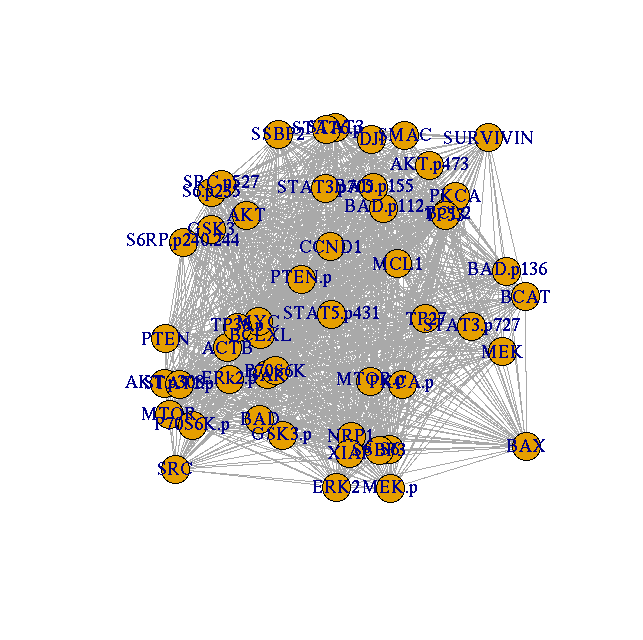
\includegraphics[width=1\linewidth]{Conditional_Density_Network.png}
    \caption{Caption}
    \label{fig:enter-label}
\end{figure}
\pagebreak
We see that this image, the nodes labeled with each relevant protein, suggest a highly dependent data set. 

In this case, a threshold value of 0.1 was used. That is, if a partial correlation was greater than 0.1, the nodes were connected on the graph. 

\subsection{Diagnostics and Variational Inference}

After completing the graph and establishing the Gibbs sampler, traditional MCMC convergence methods for a single Markov Chain were performed, in particular tests to measure convergence and mixing. 

Diagnostic results from the Gibbs sampler can be found detailed by the above plots. 
\pagebreak
% place holder for plot 1 
\bigskip
\begin{figure}
    \centering
    \includegraphics[width=0.5\linewidth]{omega_trace1.png}
    \caption{Trace Plots for Omega 1 Case Example}
    \label{fig:enter-label}
\end{figure}

%place holder for plot 2 
\pagebreak
\begin{figure}
    \centering
    \includegraphics[width=0.5\linewidth]{omega_trace2.png}
    \caption{Trace Plots for Omega 2 Case Example}
    \label{fig:enter-label}
\end{figure}

As evidenced by the plots, we found the mixing and convergence of the Markov Chain to be adequate as evidenced by trace plots from a few selections from the Precision matrix simulation, however further research and evaluation would be appropriate, for example with differing starting points or varying iterations and a fraction of the time used for the burn-in period. Comparison of various iteration lengths as well as burn-in, and even the necessity of a burn in period at all, in a type of cross-validation, we imagine would be fruitful for further analysis. 

Given the convergence of the Markov Chain as well as the diagnostic plots and undirected graph, we decided that variational inference would not be appropriate in this case. 

\section*{References}


References follow the acknowledgments in the camera-ready paper. Use unnumbered first-level heading for
the references. Any choice of citation style is acceptable as long as you are
consistent. It is permissible to reduce the font size to \verb+small+ (9 point)
when listing the references.
Note that the Reference section does not count towards the page limit.
\medskip


\small

% just replacing over the top 
[1] Griffin, J.E.\ \& Brown P.J.\ (2010) Inference with normal-gamma prior distributions in regression problems. {\it Bayesian Analysis 5(1)}:171-188.

[2] Kornblau, S.M. et al (2009) Functional proteomic profiling of aml predicts response and survival. {\it Blood, The Journal of the American Society of Hematology,} 113(1):154-164.

[3] Meinshausen N.\ \& Buhlmann P.\ (2006) High-dimensional graphs and variable selection with the lasso. {\it The Annals of Statistics,}34(3):1436-1462.

[4] Mitchell T.J.\ \& Beauchamp J.J.\ (1988) Bayesian variable selection in linear regression. {\it Journal of the American Statistical Association,}83(404):1023-1032.

[5] Piironen J.\ \& Vehtari A.\ (2017) On the hyperprior choice for the global shrinkage parameter in the horseshoe prior. {\it Artificial Intelligence and Statistics} 905-913.

[6] Wang Z. et al (2022) Bayesian edge regression in undirected graphical models to characterize interpatient heterogeneity in cancer. {\it Journal of the American Statistical Association}:533-546.

\end{document}